%\documentclass[11pt]{article}  % for e-submission to ApJ
\documentclass[11pt]{NSF}  % for e-submission to ApJ

%\documentclass[12pt,preprint2]{aastex}  % for e-submission to ApJ - two column

%\documentclass[manuscript]{emulateapj}  % this makes everything look like ApJ

\usepackage{graphicx, natbib, color, bm, amsmath, epsfig}

%paper commands, for when not using aastex
\newcommand\physrep{Phys.~Rep.}
\newcommand\fcp{Fund.~Cosmic~Phys.}
\newcommand{\pre}{Phys Rev E}
\newcommand{\apj}{ApJ}
\newcommand{\apjs}{ApJS}
\newcommand{\aj}{AJ}
\newcommand{\aap}{A\&A}
\newcommand{\mnras}{MNRAS}
\newcommand{\araa}{ARA\&A}
\newcommand{\procspie}{Proc.SPIE}
\newcommand{\pasj}{PASJ}
\newcommand{\iaucirc}{IAU Circ.}
\newcommand{\aplett}{AP Letters}
\newcommand{\aaps}{AAPS}
\newcommand{\aapr}{AAPR}
\newcommand{\nat}{Nature}
\newcommand{\apjsupp}{ApJS}
\newcommand{\pasp}{PASP}
\newcommand{\apjl}{ApJL}
\newcommand\prl{Phys.~Rev.~Lett.}
\newcommand\apss{Ap\&SS}




%%%% PUT NEW COMMANDS AND DEFINITIONS HERE %%%%
\usepackage{graphicx, natbib, color, bm, amsmath, epsfig}

%
% Hijacked and hacked from aastex.cls
%
%\def\newblock{\hskip .11em\@plus.33em\@minus.07em}%

%\newcommand\plotone[1]{%
% \typeout{Plotone included the file #1}
% \centering
% \leavevmode
% \includegraphics[width={\eps@scaling\columnwidth}]{#1}%
%}
%\newcommand\plotone[1]{
% \includegraphics[width=3.0in]{#1}%
%}
%\let\tableline=\hline
%enzo commands
\newcommand\jcompphys{J.~Comput.~Phys}
\newcommand\physfluidsa{Phys.~Fluids~A}
\newcommand\physfluids{Phys.~Fluids}
\newcommand\physlettA{Phys.~Lett.~A}
\newcommand\jfm{J.~Fluid~Mech.}
\newcommand\ccm{Comput.~Phys.~Commun.}
\newcommand\jphysique{J.~Physique~I}
\newcommand\revmodphys{Rev.~Mod.~Phys.~}

%\newcommand\aap{\ref@jnl{A\&A}}% 
%\newcommand\prb{\ref@jnl{Phys.~Rev.~B}}% 
          % Physical Review B: Solid State 


\newcommand{\ratio}{\mathcal{R}}
\newcommand{\yt}{{\tt yt}}
\newcommand{\Lmax}{\ell_{\rm max}}
\newcommand{\enzo}{{\small Enzo}}
\newcommand{\menzo}{{EnzoMHD}}
\newcommand{\Menzo}{{EnzoMHD}}
\newcommand{\zeus}{{\small ZEUS}}
\newcommand{\Lbox}{L_{\rm box}}
\newcommand{\Nroot}{N_{\rm root}}
\newcommand{\K}{\,\rm K}
\newcommand{\dave}{DaveThena}
\newcommand{\grid}{{\tt grid}}

%\newcommand{\lct}[3]{\ensuremath{\epsilon_{#1,#2,#3}}}
\newcommand{\lct}[1]{\ensuremath{\epsilon_{#1}}}
%grid location commands.
\newcommand{\iph}{i + \frac{1}{2}}
\newcommand{\imh}{i - \frac{1}{2}}
\newcommand{\jph}{j + \frac{1}{2}}
\newcommand{\jmh}{j - \frac{1}{2}}
\newcommand{\kph}{k + \frac{1}{2}}
\newcommand{\kmh}{k - \frac{1}{2}}

\newcommand{\ipmh}{i \pm \frac{1}{2}}
\newcommand{\half}{\frac{1}{2}}
\newcommand{\quart}{\frac{1}{4}}
\newcommand{\tquart}{\frac{3}{4}}

%physics commands
\newcommand{\avir}{\ensuremath{\alpha_{\rm{vir}}}}
\newcommand{\mach}{\ensuremath{\mathcal{M}}}
\newcommand{\hmag}{\ensuremath{H_{\rm{M}}}}
\newcommand{\alfmach}{\ensuremath{\mathcal{M_{\rm{A}}}}}
%\newcommand{\msun}{\ensuremath{\rm{M}_\odot}}
\newcommand{\msun}{\ensuremath{M_\odot}}
\newcommand{\lsun}{\ensuremath{L_\odot}}
\newcommand{\rsun}{\ensuremath{R_\odot}}

\def\mch{\ensuremath{M_{\rm{Ch}}}}
\def\AD{{\rm{AD}}}

%math commands
\def\rms{\ensuremath{\rm{rms}}}
\newcommand{\pts}[1]{\emph{(#1 pts)}}
\newcommand{\dbd}[2]{\frac{ \partial #1 }{ \partial #2} }
\newcommand{\ddbd}[2]{\frac{ d #1 }{ d #2} }
\newcommand{\dDbD}[2]{\frac{ \mathrm{D} #1 }{ \mathrm{D} #2} }
\newcommand{\curl}{\nabla \times}
\newcommand{\divb}{\ensuremath{\nabla \cdot {\bvec}}}
\newcommand{\divv}{\ensuremath{\nabla \cdot {\vvec}}}
\newcommand{\divbo}{$\nabla \cdot {\bf B} = 0$}
\newcommand{\intd}[1]{\int_#1^{#1 + \Delta #1} }
\newcommand{\dt}{\Delta t}
\newcommand{\dx}{\Delta x}
\newcommand{\dy}{\Delta y}
\newcommand{\dz}{\Delta z}
\newcommand{\p}[1]{#1^\prime }
\newcommand{\pp}[1]{#1^{\prime \prime} }
\newcommand{\tff}{\ensuremath{t_{\rm{ff}}}}
\newcommand{\kkmin}{\ensuremath{k/k_{\rm{min}}}}
\newcommand{\kmax}{\ensuremath{k_{\rm{max}}}}

%dcc color commands
\definecolor{orange}{rgb}{1.        ,  0.54,  0}
\newcommand{\orange}[1]{\textcolor{orange}{#1}}

\newcommand{\gtt}[1]{\textcolor{green}{{\tt#1}}}
\newcommand{\red}[1]{\textcolor{red}{#1}}
\newcommand{\yellow}[1]{\textcolor{yellow}{#1}}
\newcommand{\blue}[1]{\textcolor{blue}{#1}}
\definecolor{meta}{rgb}{0.371,0.617,0.625} %cadet blue for
                                           %non-production worthy
                                           % discussion of the work
\newcommand{\meta}[1]{\textcolor{meta}{#1}}
\newcommand{\green}[1]{\textcolor{green}{#1}}
\newcommand{\aake}[1]{\textcolor{blue}{#1}}
\newcommand{\bld}[1]{\mathbf{#1}}

\def\here{\red{notes later}}
%\newcommand{\hilite}[1]{\textcolor{red}{#1}}
%\newcommand{\hilite}[1]{#1}

%\newcommand{\bold}[1]{{\bf #1}}
%the comment maker, dc: the first one will show all comments in green, 
%the second hides them all.
%\newcommand{\dc}[1]{\textcolor{green}{#1}}
\newcommand{\dc}[1]{}
%\newcommand{\dc}[1]{#1}
%\def\bvec{\ensuremath{\vec{B}}}
%\def\vvec{\ensuremath{\vec{v}}}
\def\Bvec{\ensuremath{{\bf B}}}
\def\Jvec{\ensuremath{{\bf J}}}
\def\Avec{\ensuremath{{\bf A}}}
\def\bvec{\ensuremath{{\bf b}}}
\def\vvec{\ensuremath{{\bf v}}}
\def\uvec{\ensuremath{{\bf u}}}
\def\rvec{\ensuremath{{\bf r}}}
\def\xvec{\ensuremath{{\bf x}}}
\def\kvec{\ensuremath{{\bf k}}}
\def\Omegavec{\ensuremath{{\bf \Omega}}}
\def\omegavec{\ensuremath{{\bf \omega}}}
%\newcommand{\BlockOut}[1]{}
\newcommand{\BlockOut}[1]{#1}
\newcommand{\imp}{\ensuremath{\implies}}
\newcommand{\question}[1]{\textcolor{red}{#1}}
\definecolor{pink}{rgb}{1.        ,  0.75294118,  0.79607843}
\definecolor{maroon}{rgb}{0.69019608,  0.18823529,  0.37647059}
\newcommand{\ToRead}[1]{\textcolor{maroon}{#1}}
\newcommand{\ToReadUrgent}[1]{\textcolor{red}{#1}}
\newcommand{\HaveRead}[1]{\textcolor{black}{#1}}
\newcommand{\Old}[1]{\textcolor{blue}{#1}}
\newcommand{\Scanned}[1]{\textcolor{meta}{#1}}
\newcommand{\dccnote}[1]{}
%\newcommand{\dccnote}[1]{\textcolor{red}{#1}}
\def\nn{\nonumber}

\newcommand{\get}[1]{\textcolor{red}{#1}}
\definecolor{gray}{rgb}{0.5,0.5,0.5}
\newcommand{\gray}[1]{\textcolor{gray}{#1}}
\newcommand{\clean}[1]{\textcolor{gray}{#1}}
\newcommand{\ToDo}[1]{\textcolor{red}{#1}}
\def\etal{{\sl et al.}}

%chemistry commands
\newcommand{\Htwo}{\ensuremath{\rm{H}_2}}
\newcommand{\twelveco}{\ensuremath{^{12}\rm{CO}}}
\newcommand{\thirteenco}{\ensuremath{^{13}\rm{CO}}}

\newcommand{\mhdlabel}{{_{MHD}}}
\newcommand{\gravlabel}{{_{Grav}}}
\newcommand{\fclabel}{{_{fc}}}
\newcommand{\explabel}{{_{exp}}}
\newcommand{\sci}[1]{\ensuremath{\times {10^{#1}}}}
\newcommand{\percc}{\ensuremath{\rm{cm}^{-3}}}
\newcommand{\gcc}{\ensuremath{\rm{g}\ \rm{cm}^{-3}}}
\newcommand{\kms}{\ensuremath{\rm{km}\ \rm{s}^{-1}}}
\newcommand{\cms}{\ensuremath{\rm{cm}\ \rm{s}^{-1}}}
\newcommand{\cmperg}{\ensuremath{\rm{cm}^{2}\ \rm{g}^{-1} }}
\newcommand{\cmcmpers}{\ensuremath{\rm{cm}^2\ \rm{s}^{-1} }}
\def\muG{\ensuremath{\mu\rm{G}}}
\def\micron{\ensuremath{\mu\rm{m}}}
\def\alf{Alfv\' en}
\def\Alfvenic{Alfv\' enic}
\def\sa{super-Alfv\' enic}
\def\Sa{Super-Alfv\' enic}
\def\suba{sub-Alfv\' enic}
\def\Suba{Sub-Alfv\' enic}
\def\transa{trans-Alfv\' enic}
\def\Transa{Trans-Alfv\' enic}
\def\cs{\ensuremath{c_{\rm{s}}}}
\def\va{\ensuremath{v_{\rm{A}}}}
\def\sfrff{\ensuremath{{\rm SFR_{ff}}}}
%\def\velocity{\ensuremath{\vec{v}}}
%\def\magnetic{\ensuremath{\vec{B}}}
\def\velocity{\ensuremath{{\bf v}}}
\def\magnetic{\ensuremath{{\bf B}}}
\newcommand{\Fourier}[1]{\ensuremath{\tilde{#1}}}
\def\hfw{0.49}
\def\hw{0.49}
\def\fw{0.9}

\def\ssp{\def\baselinestretch{1.0}\large\normalsize}

\def\rhoc{\ensuremath{\rho_{\rm{c}}}}
\def\erf{\ensuremath{\rm{erf}}}


\def\tfinal{T_{\rm{final}}}
\def\suzu{\ensuremath{\rm{SU}_{\rm{zone}}}}
\def\nzones{N_{\rm{z},\ell}}
\newcommand{\Lund}{\ensuremath{\mathrm{S}}}
%\newcommand{\SUestimate}[1]{\textcolor{red}{#1}}
\newcommand{\SUestimate}[1]{#1}
\def\SUtotal{5\sci{4}}
\def\SUsn{1.9\sci{4}}
\def\SUcore{1.6\sci{4}}
\def\SUturb{1.5\sci{4}}
\def\DiskCore{1.5\sci{4} Gb}
\def\DiskSNe{1.7\sci{4}Gb}
\def\DiskTurb{3.2\sci{3} Gb}
\def\StoreTotal{3.5\sci{4} Gb}
\def\nameCores{\emph{cores}}
\def\nameSupernova{\emph{supernovae}}
\def\nameTurbulence{\emph{turbulence}}
\def\suPerZoneUpCores{\ensuremath{6.2\sci{-11}}}
\def\suPerZoneUpSupernova{\ensuremath{5.2\sci{-11}}}
\def\suPerZoneUpTurbulence{\ensuremath{4.4\sci{-11}}}

\citestyle{aa}  % correct formatting for ApJ style files

\usepackage{aas_macros}
\begin{document}

\begin{centering}
\begin{LARGE}
Scaling Information for 

``Three Projects in Astrophysical Magnetohydrodynamics''
\end{LARGE}

David Collins, PI

\end{centering}


\pagestyle{plain}

The three projects presented in this proposal will be using the code Enzo
\citep{Bryan14}.
Enzo  is an open source adaptive mesh refinement (AMR) code that
has been used in hundreds of astrophysical works.  These studies include the
formation of the first stars \citep{Abel02}, clusters of galaxies \citep{Xu11}
and the large scale structure of the universe.  It employs several hydrodynamics
solvers, including the piecewise parabolic method  \citep[PPM,][]{Colella84}, two implementations of
magnetohydrodynamics (MHD), self-gravity, and Lagrangian particles that can be used
for collisionless dark matter, stars, dust, and passive tracers.  One of the
primary advantages of Enzo over other codes is its use of structured AMR, which
allows it to add resolution elements adaptively as dictated by the problem.  A
variety of refinement criterion are available.   The present studies will use
the divergence-preserving MHD module \citep{Collins10}.  For the patch solver we
use the
second order MHD method of \citet{Li08a} and the constrained transport method of
\citet{Gardiner05} to preserve the divergence-free constraint (\divbo) to
machine precision.  For the AMR, the divergence-free reconstruction of \citet{Balsara01}
is used to interface magnetic fields with the adaptive mesh.  For chemistry and
radiative cooling used in the \emph{cores} project, Grackle is used
\citep{Smith17}.  For the burning operator in the \emph{supernova} project, we
use the implementation of \citep{Hristov18}. The \emph{turbulence} project will
use only the isothermal MHD package.


To measure the behavior of the solvers, we ran a weak scaling test with the main
physics packages for the three projects.  
A constant amount of
work, $128^3$ zones per task, was used for each node, and the refinement was forced to
occupy the inner 1/8 of the domain volume.  Scaling was done from 8 through 4096
processors, with 64 threads per node (when possible).
The packages in question do not depend heavily on the regime of
physics in question, so uniform gas was taken in each case.  The results can be
seen in Figure \ref{fig.scaling}.  Here we plot updates-per-core-second.
for ideal scaling, this will be independent of the number of nodes or zones.  

The blue curve, applicable to the \nameTurbulence\ suite, contains only the MHD
solver and random forcing.  This is extremely parallelizable, as the work is
entirely local.  The orange curve, applicable to the \nameSupernova\ project,
uses the MHD solver and nuclear burning machinery.  The performance of this
package sharply declines at 4096 threads.  
This decrease in performance will be
addressed in the near future, but does not pose a threat to the successful
completion of the simulations.  The green curve is a uniform box with MHD,
cooling, and self gravity.  Being a non-local operator, the self gravity does
not scale perfectly.  This curve is relevant for the \nameCores\ project.

If $Z$ is the number of updates-per-core-second in the Figure, the cost per
simulation in node-hours, $SU_{zu}=1/(Z*3600*N_{\rm{core-per-node}})$.  We will
use 64 threads-per-node where possible.  

\begin{figure} \begin{center}
    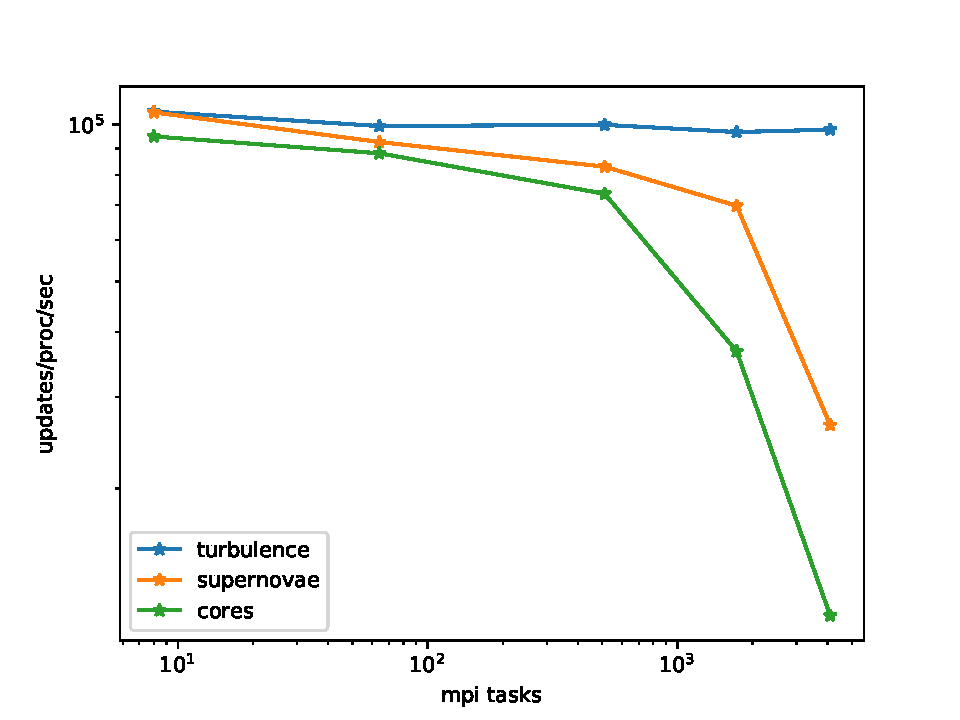
\includegraphics[width=0.99\textwidth]{g40_zoneup.pdf}
\caption[ ]{Updates per core-second for weak scaling with one level of AMR on
    Stampede 2.    The three curves correspond to the three different sets of
    physics packages for each suite of simulations.  The blue curve only employs
    the MHD solver, in the configuration used for the \nameTurbulence\
    simulations.  The orange curve employs the MHD solver as well as the burning
    operator, and will be used for the \nameSupernova\ simulations.  The green
    curve employs self gravity and cooling, and will be used for the \nameCores\
    simulations.
    }
\label{fig.scaling} \end{center} \end{figure}



\bibliographystyle{apj}
\bibliography{apj-jour,ms.bib}  % looks in ms.bib for bibliography info

\end{document}  


